% =====================================================================
%  limites-y-continuidad.tex — CDIV — Límites y continuidad (Teórico)
%  Requiere apuntes.sty (estilo/ en la raíz del repo; ver README).
% =====================================================================
\documentclass[11pt,a4paper]{article}
\usepackage{apuntes}

% ---------- Macros propias de esta materia (solo si hacen falta) ----------
\newcommand{\Rbar}{\overline{\R}}
\newcommand{\Er}{E^{*}}                 % entorno reducido
\newcommand{\Int}[1]{\mathring{#1}}     % interior
\newcommand{\Cl}[1]{\overline{#1}}      % clausura
\newcommand{\cE}{\mathcal{E}}           % familia de entornos

% ---------- Metadatos ----------
\materia{CDIV}
\curso{Teórico}
\unidad{Límites y continuidad}
\periodo{Clases 18 a 28 --- 2026}
\hypersetup{pdfauthor={Santiago Trujillo}}

\begin{document}
\maketitle
\vspace{-1.6em}
\begin{center}
  {\normalsize Santiago Trujillo\par}
\end{center}
\vspace{0.5em}
\tableofcontents

% =====================================================================
%  CLASES — cada clase nueva se agrega AL FINAL, sin tocar las anteriores
% =====================================================================

% Las hojas de las clases 18 a 24 no tienen fecha: el campo queda vacío.
\clase{18}{}{Entornos y límite}

\subsection{Introducción}

\subsubsection*{Entorno}

\begin{definicion}
Sean $x_0\in\R$ y $\varepsilon>0$.
\begin{itemize}
  \item El entorno de centro $x_0$ y de radio $\varepsilon$ es el conjunto
  \begin{align*}
    E(x_0,\varepsilon) &:= \{x\in\R : \abs{x-x_0}<\varepsilon\}\\
    &= (x_0-\varepsilon,\, x_0+\varepsilon).
  \end{align*}
  \item El entorno reducido de centro $x_0$ y de radio $\varepsilon>0$ por
  \begin{align*}
    \Er(x_0,\varepsilon) &:= E(x_0,\varepsilon)\setminus\{x_0\}\\
    &= \{x\in\R : 0<\abs{x-x_0}<\varepsilon\}\\
    &= (x_0-\varepsilon,\, x_0)\cup(x_0,\, x_0+\varepsilon).
  \end{align*}
\end{itemize}
\end{definicion}

\begin{observacion}
$0<\varepsilon'<\varepsilon \implies E(x_0,\varepsilon')\subset E(x_0,\varepsilon)$ y $\Er(x_0,\varepsilon')\subset \Er(x_0,\varepsilon)$.
\end{observacion}

\begin{definicion}
Sea un intervalo $I\subset\R$.
\begin{itemize}
  \item El interior de $I$ es el subintervalo $\Int{I}\subset I$ obtenido excluyendo los extremos de $I$.
  \item La clausura de $I$ es el sobreintervalo $\Cl{I}\supset I$ obtenido incluyendo los extremos finitos de $I$.
\end{itemize}
\end{definicion}

\begin{center}
\renewcommand{\arraystretch}{1.3}
\begin{tabular}{l|c|c}
\toprule
Intervalo $I$ & Interior $\Int{I}$ & Clausura $\Cl{I}$ \\
\midrule
$[a,b],\ (a,b],\ [a,b),\ (a,b)$ \quad con $a<b$ & $(a,b)$ & $[a,b]$ \\
$(-\infty,a],\ (-\infty,a)$ & $(-\infty,a)$ & $(-\infty,a]$ \\
$[a,+\infty),\ (a,+\infty)$ & $(a,+\infty)$ & $[a,+\infty)$ \\
$(-\infty,+\infty)=\R$ & $\R$ & $\R$ \\
$\{a\}\ (=[a,a])$ & $\emptyset$ & $\{a\}$ \\
$\emptyset$ & $\emptyset$ & $\emptyset$ \\
\bottomrule
\end{tabular}
\end{center}

\begin{observacion}
$\Int{I}\subset I\subset \Cl{I}$.
\end{observacion}

\textbf{Vocabulario:}
\begin{itemize}
  \item $x$ es interior de $I$ si $x\in\Int{I}$.
  \item $x$ es adherente a $I$ si $x\in\Cl{I}$.
\end{itemize}

\begin{proposicion}
Dados $I\subset\R$ y $x\in\R$:
\begin{itemize}
  \item $x\in\Int{I} \iff \exists\,\varepsilon>0,\ E(x,\varepsilon)\subset I$.
  \item $x\in\Cl{I} \iff \forall\,\varepsilon>0,\ E(x,\varepsilon)\cap I\neq\emptyset$.
\end{itemize}
\end{proposicion}

\begin{convencion}
En lo que sigue, solo consideraremos funciones definidas en intervalos $I$ cuyo interior no es vacío; $\Int{I}\neq\emptyset$.
\end{convencion}

\begin{proposicion}
Si $I\subset\R$ es un intervalo tal que $\Int{I}\neq\emptyset$, entonces:
\[
  \forall x_0\in\Cl{I},\ \forall\varepsilon>0,\quad \Er(x_0,\varepsilon)\cap I\neq\emptyset.
\]
\end{proposicion}

\subsection{Límites}

\begin{definicion}
Sean $f:I\to\R$, $x_0\in\Cl{I}$ y $L\in\R$. Se escribe:
\[
  f(x)\xrightarrow[x\to x_0]{} L \qquad\text{(``$f(x)$ tiende a $L$ cuando $x$ tiende a $x_0$'')}
\]
o
\[
  \lim_{x\to x_0} f(x) = L \qquad\text{(``$f$ tiene límite $L$ en el punto $x_0$'')}
\]
cuando:
\[
  \forall\varepsilon>0,\ \exists\delta>0,\ \forall x\in I,\quad 0<\abs{x-x_0}<\delta \implies \abs{f(x)-L}<\varepsilon.
\]
\end{definicion}

\begin{observacion}
(1) Con los entornos, la definición se escribe
\begin{align*}
  &\forall\varepsilon>0,\ \exists\delta>0,\ \forall x\in\Er(x_0,\delta)\cap I,\ f(x)\in E(L,\varepsilon)\\
  \iff\ &\forall\varepsilon>0,\ \exists\delta>0,\ f\big(\Er(x_0,\delta)\cap I\big)\subset E(L,\varepsilon).
\end{align*}
\end{observacion}

\begin{idea}
La definición expresa que $f(x)$ es arbitrariamente cercano a $L$ en cuanto $x$ sea suficientemente cercano a $x_0$.
\begin{itemize}
  \item $\forall\varepsilon>0,\ \exists\delta>0$: ``para toda precisión $\varepsilon>0$, existe un radio $\delta>0$''.
  \item $\forall x\in\Er(x_0,\delta)\cap I$: si $x$ es cercano a $x_0$ (a menos de $\delta$),
  \item $f(x)\in E(L,\varepsilon)$: entonces $f(x)$ es cercano a $L$ a menos de $\varepsilon$.
\end{itemize}
\end{idea}

\begin{center}
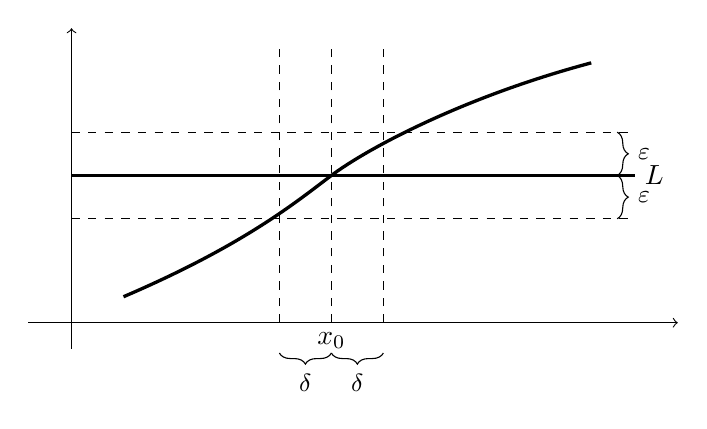
\begin{tikzpicture}[scale=1.1]
  \draw[->] (-0.5,0) -- (7,0);
  \draw[->] (0,-0.3) -- (0,3.4);
  \draw[dashed] (0,1.2) -- (6.5,1.2);
  \draw[thick] (0,1.7) -- (6.5,1.7) node[right] {$L$};
  \draw[dashed] (0,2.2) -- (6.5,2.2);
  \draw[decorate,decoration={brace,amplitude=4pt}] (6.3,2.2) -- (6.3,1.7) node[midway,right=4pt] {\small$\varepsilon$};
  \draw[decorate,decoration={brace,amplitude=4pt}] (6.3,1.7) -- (6.3,1.2) node[midway,right=4pt] {\small$\varepsilon$};
  \draw[dashed] (2.4,0) -- (2.4,3.2);
  \draw[dashed] (3,0) -- (3,3.2);
  \draw[dashed] (3.6,0) -- (3.6,3.2);
  \node[below] at (3,0) {$x_0$};
  \draw[decorate,decoration={brace,amplitude=4pt,mirror}] (2.4,-0.35) -- (3,-0.35) node[midway,below=4pt] {\small$\delta$};
  \draw[decorate,decoration={brace,amplitude=4pt,mirror}] (3,-0.35) -- (3.6,-0.35) node[midway,below=4pt] {\small$\delta$};
  \draw[very thick] (0.6,0.3) .. controls (2,0.9) and (2.6,1.4) .. (3,1.7) .. controls (3.4,2.0) and (4.5,2.6) .. (6,3.0);
\end{tikzpicture}
\end{center}

% NOTA: el escaneo pasa de la observación (1) a la (3); la (2) no figura.
\begin{observacion}
(3) El valor de $f(x_0)$ (cuando existe) no influye ni en la existencia de límite, ni en su valor.
\end{observacion}

\begin{proposicion}
Sean $f:I\to\R$ y $x_0\in\Cl{I}$. Si $f(x)\xrightarrow[x\to x_0]{}L$ y $f(x)\xrightarrow[x\to x_0]{}L'$, entonces $L=L'$.
\end{proposicion}

\begin{demo}
Por el absurdo, supongamos que $L\neq L'$. Sea $\varepsilon := \dfrac{\abs{L-L'}}{2} > 0$.
\begin{itemize}
  \item Como $f(x)\xrightarrow[x\to x_0]{}L$, existe $\delta>0$ tal que $\forall x\in\Er(x_0,\delta)\cap I,\ f(x)\in E(L,\varepsilon)$.
  \item Como $f(x)\xrightarrow[x\to x_0]{}L'$, existe $\delta'>0$ tal que $\forall x\in\Er(x_0,\delta')\cap I,\ f(x)\in E(L',\varepsilon)$.
\end{itemize}
Se fija $x\in\Er\big(x_0,\min(\delta,\delta')\big)\cap I$.

Luego: $f(x)\in E(L,\varepsilon)$ y $f(x)\in E(L',\varepsilon)$, absurdo, pues ambos conjuntos no se intersectan.
\end{demo}

\begin{observacion}
En el caso donde $x_0\in I$, existen esencialmente 3 situaciones posibles:
\begin{itemize}
  \item o bien $f$ no tiene límite en $x_0$,
  \item o bien $f$ tiene límite $L\neq f(x_0)$ en $x_0$,
  \item o bien $f$ tiene límite $L=f(x_0)$.
\end{itemize}
En el último caso, se dice que $f$ es continua en el punto $x_0$.
\end{observacion}

% =====================================================================
\clase{19}{}{Continuidad y ejemplos}

Dados:
\begin{itemize}
  \item una función $f:I\to\R$,
  \item un punto $x_0\in\Cl{I}$,
  \item un número $L\in\R$,
\end{itemize}
\[
  \lim_{x\to x_0}f(x)=L \ \overset{\text{def}}{\iff}\ \forall\varepsilon>0,\ \exists\delta>0,\ \forall x\in I,\ \underbrace{0<\abs{x-x_0}<\delta}_{x\in\Er(x_0,\delta)} \implies \underbrace{\abs{f(x)-L}<\varepsilon}_{f(x)\in E(L,\varepsilon)}.
\]

\begin{definicion}
$f:I\to\R$ es continua en un punto $x_0\in I$ si $\displaystyle\lim_{x\to x_0}f(x)=f(x_0)$ (existe).
\end{definicion}

\begin{definicion}
$f$ es continua en $I$ si es continua en todo punto $x_0\in I$.
\end{definicion}

\subsection{Ejemplos}

\begin{ejemplo}[Identidad]
Sea $f(x)=x$ ($x\in\R$). Entonces para todo $x_0\in\R$, $\displaystyle\lim_{x\to x_0}f(x)=x_0\ (=f(x_0))$.

Sea $\varepsilon>0$. Se define $\delta_\varepsilon:=\varepsilon>0$. Sea $x\in\R$ tal que $0<\abs{x-x_0}<\delta_\varepsilon$. Tenemos que $\abs{x-x_0}<\varepsilon$, es decir $\abs{f(x)-x_0}<\varepsilon$.
\end{ejemplo}

\begin{ejemplo}
Sea $f:[0,+\infty)\to\R$ definida por $f(x)=\sqrt{x}$ (para todo $x\geq 0$). Entonces, $\forall x_0\in[0,+\infty)$, $\displaystyle\lim_{x\to x_0}f(x)=\sqrt{x_0}\ (=f(x_0))$.

\textbf{Caso $x_0=0$.} Se define $\delta_\varepsilon:=\varepsilon^2>0$ ($\forall\varepsilon>0$). Sea $x\in[0,+\infty)$ tal que $0<\abs{x-0}<\delta_\varepsilon$, es decir $0<x<\varepsilon^2\ (=\delta_\varepsilon)$; entonces $0<\sqrt{x}<\sqrt{\varepsilon^2}=\varepsilon$, entonces $\abs{\sqrt{x}-0}<\varepsilon$.

\textbf{Caso $x_0>0$.} Sea $\varepsilon>0$. Se definen $\varepsilon':=\min(\varepsilon,\sqrt{x_0})>0$ y
\begin{center}
$\displaystyle\delta_\varepsilon := \min\Big( (\sqrt{x_0}+\varepsilon')^2-x_0,\ x_0-(\sqrt{x_0}-\varepsilon')^2 \Big) > 0$
\end{center}
Sea $x\in[0,+\infty)$ tal que $0<\abs{x-x_0}<\delta_\varepsilon$. Sabemos que:
\begin{itemize}
  \item $x < x_0+\delta_\varepsilon \leq x_0 + \big((\sqrt{x_0}+\varepsilon')^2-x_0\big) = (\sqrt{x_0}+\varepsilon')^2$,
  \item $x > x_0-\delta_\varepsilon \geq x_0 - \big(x_0-(\sqrt{x_0}-\varepsilon')^2\big) = (\sqrt{x_0}-\varepsilon')^2$.
\end{itemize}
Luego:
\begin{align*}
  (\sqrt{x_0}-\varepsilon')^2 &< x < (\sqrt{x_0}+\varepsilon')^2\\
  \sqrt{x_0}-\varepsilon' &< \sqrt{x} < \sqrt{x_0}+\varepsilon'\\
  \abs{\underbrace{\sqrt{x}}_{f(x)}-\underbrace{\sqrt{x_0}}_{L}} &< \varepsilon' \leq \varepsilon.
\end{align*}
\end{ejemplo}

\begin{observacion}
Vimos que
\[
  f(x)\xrightarrow[x\to x_0]{}L \iff \forall\varepsilon>0,\ \exists\delta>0,\ \forall x\in\Er(x_0,\delta),\ f(x)\in E(L,\varepsilon).
\]
Entonces
\[
  f(x)\ \not\!\!\xrightarrow[x\to x_0]{}L \iff \exists\varepsilon>0,\ \forall\delta>0,\ \exists x\in\Er(x_0,\delta),\ \abs{f(x)-L}\geq\varepsilon.
\]
En particular: $f$ no tiene límite en $x_0\in\Cl{I}$ si y sólo si
\[
  \forall L\in\R,\ \exists\varepsilon>0,\ \forall\delta>0,\ \exists x\in\Er(x_0,\delta),\ \abs{f(x)-L}\geq\varepsilon.
\]
\end{observacion}

\begin{contraejemplo}
$\sgn:\R\to\R$ definida por
\[
  \sgn(x)=\begin{cases} 1 & \text{si } x>0,\\ 0 & \text{si } x=0,\\ -1 & \text{si } x<0.\end{cases}
\]
\begin{center}
\begin{tikzpicture}[scale=0.9]
  \draw[->] (-3,0) -- (3,0);
  \draw[->] (0,-1.6) -- (0,1.6);
  \draw[very thick] (-2.8,-1) -- (0,-1);
  \draw[very thick] (0,1) -- (2.8,1);
  \draw[fill=white] (0,-1) circle (2pt);
  \draw[fill=white] (0,1) circle (2pt);
  \fill (0,0) circle (2pt);
\end{tikzpicture}
\end{center}
\end{contraejemplo}

\begin{proposicion}
La función signo no tiene límite en $x_0=0$.
\end{proposicion}

\begin{demo}
Se trata de demostrar que:
\[
  \forall L\in\R,\ \exists\varepsilon>0,\ \forall\delta>0,\ \exists x\in\R,\ 0<\abs{x}<\delta \ \wedge\ \abs{\sgn(x)-L}\geq\varepsilon
\]
\comentario{el $\wedge$ se lee ``pero''}.

Sea $L\in\R$. Se toma $\varepsilon:=1$. Sea $\delta>0$ cualquiera. Se distinguen 2 casos:
\begin{itemize}
  \item $L\geq 0$. Se toma $x:=-\delta/2$. Por construcción: $0<\abs{x}<\delta$. Pero
  \[ \abs{\sgn(x)-L} = \abs{-1-L} = \abs{L+1} = L+1 \geq 1 = \varepsilon. \]
  \item $L<0$. Se toma $x:=\delta/2$. Por construcción: $0<\abs{x}<\delta$. Pero
  \[ \abs{\sgn(x)-L} = \abs{1-L} = 1-L > 1 = \varepsilon. \qedhere \]
\end{itemize}
\end{demo}

% =====================================================================
\clase{20}{}{Propiedades algebraicas de límites}

\subsection{Propiedades algebraicas}

\begin{observacion}
Dados una función $f:I\to\R$, un punto $x_0\in\Cl{I}$ y $L\in\R$, tenemos que:
\begin{align*}
  \text{(1)}\ \lim_{x\to x_0}f(x)=L
  &\iff \text{(2)}\ \lim_{x\to x_0}\big(f(x)-L\big)=0\\
  &\iff \text{(3)}\ \lim_{x\to x_0}\abs{f(x)-L}=0.
\end{align*}
\end{observacion}

\begin{demo}
\begin{enumerate}[label=(\arabic*)]
  \item $\forall\varepsilon>0,\ \exists\delta>0,\ \forall x\in\Er(x_0,\delta)\cap I,\ \abs{f(x)-L}<\varepsilon$
  \item $\forall\varepsilon>0,\ \exists\delta>0,\ \forall x\in\Er(x_0,\delta)\cap I,\ \abs{(f(x)-L)-0}<\varepsilon$
  \item $\forall\varepsilon>0,\ \exists\delta>0,\ \forall x\in\Er(x_0,\delta)\cap I,\ \abs{\abs{f(x)-L}-0}<\varepsilon$ \qedhere
\end{enumerate}
\end{demo}

\begin{proposicion}
Sean $f,g:I\to\R$, y un punto $x_0\in\Cl{I}$. Si $\displaystyle\lim_{x\to x_0}f(x)=L$ y $\displaystyle\lim_{x\to x_0}g(x)=L'$, entonces
\[
  \lim_{x\to x_0}\big(f(x)+g(x)\big)=L+L', \qquad \lim_{x\to x_0}\big(f(x)-g(x)\big)=L-L'.
\]
\end{proposicion}

\begin{demo}[Demostración (caso de la suma)]
Por hipótesis, existen dos funciones $\varepsilon\mapsto\delta_\varepsilon$ (para $f$) y $\varepsilon\mapsto\delta'_\varepsilon$ (para $g$) tales que, para todo $\varepsilon>0$:
\begin{align*}
  \forall x\in\Er(x_0,\delta_\varepsilon)\cap I,&\quad \abs{f(x)-L}<\varepsilon \tag{$*$}\\
  \forall x\in\Er(x_0,\delta'_\varepsilon)\cap I,&\quad \abs{g(x)-L'}<\varepsilon \tag{$*'$}
\end{align*}
Se trata de construir $\varepsilon\mapsto\delta''_\varepsilon$ tal que
\[
  \forall x\in\Er(x_0,\delta''_\varepsilon)\cap I,\quad \abs{f(x)+g(x)-(L+L')}<\varepsilon.
\]
Se define $\delta''_\varepsilon := \min\big(\delta_{\varepsilon/2},\ \delta'_{\varepsilon/2}\big)$ para todo $\varepsilon>0$.

Sean $\varepsilon>0$ y $x\in I$ tal que $0<\abs{x-x_0}<\delta''_\varepsilon$. Se observa que:
\begin{itemize}
  \item $0<\abs{x-x_0}<\delta_{\varepsilon/2}$ (pues $\delta''_\varepsilon\leq\delta_{\varepsilon/2}$); entonces, por $(*)$, $\abs{f(x)-L}<\varepsilon/2$.
  \item $0<\abs{x-x_0}<\delta'_{\varepsilon/2}$ (pues $\delta''_\varepsilon\leq\delta'_{\varepsilon/2}$); entonces, por $(*')$, $\abs{g(x)-L'}<\varepsilon/2$.
\end{itemize}
Luego
\begin{align*}
  \abs{f(x)+g(x)-(L+L')} &= \abs{(f(x)-L)+(g(x)-L')}\\
  &\leq \abs{f(x)-L} + \abs{g(x)-L'} < \frac{\varepsilon}{2}+\frac{\varepsilon}{2} = \varepsilon. \qedhere
\end{align*}
\end{demo}

\begin{definicion}
Sean $f:I\to\R$ y $x_0\in\Cl{I}$. Se dice que $f$ está acotada en un entorno de $x_0$ cuando
\[
  \exists r>0,\ \exists M\geq 0\ (>0),\ \forall x\in E(x_0,r)\cap I,\quad \abs{f(x)}\leq M.
\]
\end{definicion}

\begin{lema}
Si $f$ tiene límite (finito) en $x_0$, entonces está acotada en un entorno de $x_0$.
\end{lema}

\begin{demo}
Sea $\delta>0$ tal que $\forall x\in\Er(x_0,\delta)\cap I$, $\abs{f(x)-L}<1$. Se observa que $\forall x\in\Er(x_0,\delta)\cap I$, tenemos que
\[
  \abs{f(x)} = \abs{L+(f(x)-L)} \leq \abs{L}+\abs{f(x)-L} < \abs{L}+1.
\]
\begin{itemize}
  \item Caso $x_0\in I$. Se toman $r:=\delta$ y $M=\max\big(\abs{L}+1,\ \abs{f(x_0)}\big)$.
  \item Caso $x_0\notin I$. Se toman $r:=\delta$ y $M=\abs{L}+1$. \qedhere
\end{itemize}
\end{demo}

\begin{proposicion}
Sean $f,g:I\to\R$ y un punto $x_0\in\Cl{I}$. Si
\begin{itemize}
  \item $f$ está acotada en un entorno de $x_0$,
  \item $\displaystyle\lim_{x\to x_0}g(x)=0$,
\end{itemize}
entonces $\displaystyle\lim_{x\to x_0}f(x)\cdot g(x)=0$.
\end{proposicion}

\begin{demo}
$f$ acotada localmente $\to$ $\exists r>0,\ \exists M>0,\ \forall x\in E(x_0,r)\cap I,\ \abs{f(x)}\leq M$.

$\displaystyle\lim_{x\to x_0}g(x)=0$ $\leadsto$ $\varepsilon\mapsto\delta_\varepsilon$ para $g$: $\forall x\in\Er(x_0,\delta_\varepsilon)\cap I,\ \abs{g(x)}<\varepsilon$.

Sea $\delta'_\varepsilon := \min\big(\delta_{\varepsilon/M},\ r\big)$.
\[
  \forall x\in\Er(x_0,\delta'_\varepsilon)\cap I,\quad \abs{f(x)g(x)} = \abs{f(x)}\cdot\abs{g(x)} < M\cdot\frac{\varepsilon}{M} = \varepsilon. \qedhere
\]
\end{demo}

\begin{contraejemplo}[$I=\R^+$]
$f(x)=\dfrac1x$, \quad $g(x)=x\xrightarrow[x\to0]{}0$, \quad $f(x)\,g(x)=1\ \not\!\!\xrightarrow[x\to0]{}0$.
\end{contraejemplo}

\begin{proposicion}
Si $\displaystyle\lim_{x\to x_0}f(x)=L$ y $\displaystyle\lim_{x\to x_0}g(x)=L'$, entonces $\displaystyle\lim_{x\to x_0}f(x)g(x)=LL'$.
\end{proposicion}

\begin{demo}
Se observa que
\[
  f(x)\,g(x)-LL' = \big(f(x)-L\big)L' + f(x)\big(g(x)-L'\big). \qedhere
\]
\end{demo}

\begin{proposicion}
Sea $f:I\to\R$ tal que:
\begin{itemize}
  \item $f(x)\neq0$ $\forall x\in I$,
  \item $\displaystyle\lim_{x\to x_0}f(x)=L\neq0$.
\end{itemize}
Entonces: $\displaystyle\lim_{x\to x_0}\frac{1}{f(x)}=\frac1L$.
\[
  \frac{1}{f(x)}-\frac1L = \frac{L-f(x)}{f(x)\,L}
  = -\frac1L\cdot\underbrace{\frac{1}{f(x)}}_{\substack{\text{Lema: localmente}\\\text{acotado}}}\cdot\underbrace{\big(f(x)-L\big)}_{\to\,0}\ \to\ 0.
\]
\end{proposicion}

\begin{proposicion}
Si $\displaystyle\lim_{x\to x_0}f(x)=L$ y $\displaystyle\lim_{x\to x_0}g(x)=L'\neq0$, entonces $\displaystyle\lim_{x\to x_0}f(x)/g(x)=L/L'$.
\end{proposicion}

% =====================================================================
\clase{21}{}{Cociente, monotonía y composición}

\subsection{Propiedades algebraicas}

\begin{proposicion}\label{prop:inversa}
Sea $f:I\to\R$, y $x_0\in\Cl{I}$. Si:
\begin{itemize}
  \item $f(x)\neq0$ para todo $x\in I$,
  \item $\displaystyle\lim_{x\to x_0}f(x)=L\neq0$,
\end{itemize}
entonces $\displaystyle\lim_{x\to x_0}\frac{1}{f(x)}=\frac1L$.
\end{proposicion}

\begin{corolario}
Sean $f,g:I\to\R$, y $x_0\in\Cl{I}$. Si $g(x)\neq0$ para todo $x\in I$, si $\displaystyle\lim_{x\to x_0}f(x)=L\in\R$, si $\displaystyle\lim_{x\to x_0}g(x)=L'\neq0$, entonces:
\[
  \lim_{x\to x_0}\frac{f(x)}{g(x)}=\frac{L}{L'}.
\]
\end{corolario}

\begin{demo}[Demostración de la Proposición~\ref{prop:inversa}]
Se observa que $\forall x\in I$:
\[
  \frac{1}{f(x)}-\frac1L = \frac{L-f(x)}{f(x)\,L} = -\frac1L\cdot\frac{1}{f(x)}\cdot\underbrace{\big(f(x)-L\big)}_{\xrightarrow[x\to x_0]{}0}.
\]
Sea $\varepsilon=\dfrac{\abs{L}}{2}>0$. Como $f(x)\xrightarrow[x\to x_0]{}L$, existe $\delta>0$ tal que
\[
  \forall x\in\Er(x_0,\delta),\quad \abs{f(x)-L}<\varepsilon.
\]
Para todo $x\in\Er(x_0,\delta)$, se observa que:
\begin{align*}
  \abs{L} &= \abs{f(x)-(f(x)-L)}\\
  &\leq \abs{f(x)}+\abs{f(x)-L} < \abs{f(x)}+\underbrace{\frac{\abs{L}}{2}}_{\varepsilon}\\
  \abs{f(x)} &> \abs{L}-\frac{\abs{L}}{2} = \frac{\abs{L}}{2}\\
  \abs*{\frac{1}{f(x)}} &< \frac{2}{\abs{L}}\qquad\forall x\in\Er(x_0,\delta).
\end{align*}
Luego:
\[
  \abs*{\frac{1}{f(x)}} < \max\left(\frac{2}{\abs{L}},\ \frac{1}{\abs{f(x_0)}}\right)\quad\text{en } E(x_0,\delta)\cap I. \qedhere
\]
\end{demo}

\begin{observacion}
Sea $f:\R\to\R$ definida por $f(x)=\begin{cases}\abs{x} & \text{si } x\neq0,\\ 1 & \text{si } x=0.\end{cases}$

\begin{center}
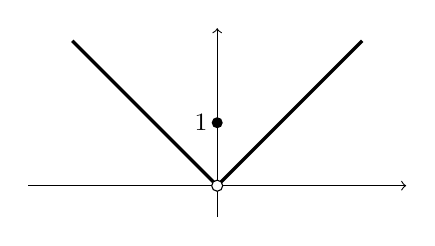
\begin{tikzpicture}[scale=0.8]
  \draw[->] (-3,0) -- (3,0);
  \draw[->] (0,-0.5) -- (0,2.5);
  \draw[very thick] (-2.3,2.3) -- (0,0) -- (2.3,2.3);
  \draw[fill=white] (0,0) circle (2.5pt);
  \fill (0,1) circle (2.5pt);
  \node[left] at (0,1) {\small$1$};
\end{tikzpicture}
\end{center}

$f(x)>0$ $\forall x\in\R$. Pero: $\displaystyle\lim_{x\to0}f(x)=0$.
\end{observacion}

\textbf{Recordatorio:}
\begin{align*}
  \lim(f+g) &= \lim f+\lim g\\
  \lim(f-g) &= \lim f-\lim g\\
  \lim fg &= \lim f\times\lim g\\
  \lim\frac fg &= \frac{\lim f}{\lim g}\quad\text{si } \lim g\neq0
\end{align*}

\begin{ejercicio}
Demostrar que si $f$ es continua y $g$ es discontinua, entonces $f+g$ es discontinua.
\end{ejercicio}

\begin{solucion}
Por el absurdo, supongamos que $f+g$ fuera continua. Luego: $\underbrace{(f+g)-f}_{g}$ es continua: absurdo.
\end{solucion}

Sea $D$ una función discontinua:
\[
  D+D=2D, \qquad D+(-D)=0.
\]

\subsection{Propiedades de monotonía}

\begin{lema}
Sea $f:I\to\R$ tal que $f(x)\geq0$ para todo $x\in I$ ($f\geq0$). Si $f$ tiene límite en un punto $x_0\in\Cl{I}$ entonces $\displaystyle\lim_{x\to x_0}f(x)\geq0$.
\end{lema}

\begin{corolario}
Si $f,g:I\to\R$ son tales que $f\leq g$ en $I$, y si tienen límites en $x_0\in\Cl{I}$, entonces $\displaystyle\lim_{x\to x_0}f(x)\leq\lim_{x\to x_0}g(x)$.
\end{corolario}

\subsubsection*{Teorema del sándwich}

\begin{teorema}[Teorema del sándwich]
Sean $f,g_1,g_2:I\to\R$ tales que $g_1(x)\leq f(x)\leq g_2(x)$ $\forall x\in I$. Dado un punto $x_0\in I$, si $g_1$ y $g_2$ tienen el mismo límite $L$ en el punto $x_0$, entonces $f$ también tiene el mismo límite en $x_0$.
\end{teorema}

\begin{ejemplo}
Sea $f:\R\to\R$ definida por $f(x)=\begin{cases}x & \text{si } x\in\Q,\\ -x & \text{si } x\notin\Q.\end{cases}$

Se observa que $-\abs{x}\leq f(x)\leq\abs{x}$ $\forall x\in\R$.
\end{ejemplo}

\begin{ejemplo}
Se recuerda que
\[
  \log(x) := \int_1^x\frac{\dd t}{t}\qquad\forall x>0.
\]
En particular: $\log 1=0$. Ya vimos que:
\[
  \underbrace{1-\frac1x}_{\to\,0} \ \leq\ \underbrace{\log x}_{\to\,0}\ \leq\ \underbrace{x-1}_{\to\,0}\qquad\forall x>0.
\]
Conclusión: $\displaystyle\lim_{x\to1}\log(x)=0=\log(1)$; $\log$ es continua en $x_0=1$.
\end{ejemplo}

\subsection{Composición de funciones}

Sean $f:I\to\R$ y $g:J\to\R$ tales que $f(I)\subset J$, es decir $\forall x\in I,\ f(x)\in J$. En esta situación, se puede definir
\[
  g\circ f:I\to\R \quad\text{por}\quad (g\circ f)(x)=g\big(f(x)\big)\quad\forall x\in I.
\]

\begin{proposicion}
Si $x_0\in\Cl{I}$, si $\displaystyle\lim_{x\to x_0}f(x)=y_0\in J$ y si $g$ es continua en $y_0\ (\in J)$, entonces $\displaystyle\lim_{x\to x_0}(g\circ f)(x)=g(y_0)$.
\end{proposicion}

\textbf{Caso particular:} si $f$ es continua en $x_0\in I$ y $g$ continua en $y_0=f(x_0)\in J$, entonces $g\circ f$ es continua en $x_0$.

% =====================================================================
\clase{22}{}{Composición y límites generalizados}

\subsection{Composición de límites}

$f:I\to\R$, $g:J\to\R$ tales que $f(I)\subset J$.
\[
  g\circ f:I\to\R,\qquad x\mapsto(g\circ f)(x)=g\big(f(x)\big).
\]

\begin{proposicion}
Si $x_0\in\Cl{I}$, si $\displaystyle\lim_{x\to x_0}f(x)=y_0$ con $\in J$ y $\displaystyle\lim_{y\to y_0}g(y)=g(y_0)$ ($g$ continua en $y_0$), entonces $\displaystyle\lim_{x\to x_0}(g\circ f)(x)=g(y_0)$.
\end{proposicion}

\begin{corolario}
Si $f$ es continua en $x_0\in I$ y $g$ es continua en $y_0=f(x_0)\in J$, entonces $g\circ f$ es continua en $x_0$.
\end{corolario}

\begin{contraejemplo}
$f,g:\R\to\R$, \quad $f(x)=0$, \quad $g(y)=\begin{cases}1 & \text{si } y=0,\\ 0 & \text{si } y\neq0.\end{cases}$

Se observa que si $x_0=y_0=0$:
\[
  \lim_{x\to x_0}f(x)=0=y_0,\qquad \lim_{y\to y_0}g(y)=0.
\]
Pero: $(g\circ f)(x)=g(f(x))=g(0)=1$. Luego $\displaystyle\lim_{x\to x_0}(g\circ f)(x)=1\neq0$.
\end{contraejemplo}

\begin{ejemplo}[Continuidad de $\log:\R^+\to\R$]
Ya sabemos que $\log$ es continua en $1$. Queremos demostrar que $\log$ es continua en cualquier punto $x_0\in\R^+$. Sea $x_0\in\R^+$ fijado:

Sea $f:\R^+\to\R$ definida por $f(x)=\dfrac{x}{x_0}$, continua. En particular $\displaystyle\lim_{x\to x_0}f(x)=1=f(x_0)$.

Sea $g:\R^+\to\R$ definida por $g(x)=\log(f(x))=\log\dfrac{x}{x_0}$. Por composición: $g=\log\circ f$ es continua en $x_0$. Pero se observa que
\begin{align*}
  \log(x) &= \log\left(\frac{x}{x_0}\right)+\log(x_0)\\
  &= g(x)+\log(x_0)\ \xrightarrow[x\to x_0]{}\ \log(x_0).
\end{align*}
\end{ejemplo}

\subsection{Generalización de la noción de límite}

\begin{notacion}
Dado un real $a\in\R$, se definen:
\begin{align*}
  \cE(a) &= \{E(a,\varepsilon):\varepsilon>0\} = \{(a-\varepsilon,\, a+\varepsilon):\varepsilon\in\R^+\}\\
  \cE^*(a) &= \{\Er(a,\varepsilon):\varepsilon>0\} = \{(a-\varepsilon,\, a)\cup(a,\, a+\varepsilon):\varepsilon\in\R^+\}
\end{align*}
\end{notacion}

\begin{observacion}
Dados $f:I\to\R$, $x_0\in\Cl{I}$, $L\in\R$, tenemos que:
\begin{align*}
  \lim_{x\to x_0}f(x)=L
  &\iff \forall\varepsilon>0,\ \exists\delta>0,\ \forall x\in I,\ 0<\abs{x-x_0}<\delta\implies\abs{f(x)-L}<\varepsilon\\
  &\iff \forall\varepsilon>0,\ \exists\delta>0,\ \forall x\in\Er(x_0,\delta)\cap I,\ f(x)\in E(L,\varepsilon)\\
  &\iff \forall\varepsilon>0,\ \exists\delta>0,\ f\big(\underbrace{\Er(x_0,\delta)}_{E}\cap I\big)\subset\underbrace{E(L,\varepsilon)}_{F}\\
  &\iff \forall F\in\cE(L),\ \exists E\in\cE^*(x_0),\ f(E\cap I)\subset F.
\end{align*}
\end{observacion}

Se consideran las siguientes nociones de entorno:
\begin{enumerate}
  \item Entorno de $a\in\R$, definido por $\cE(a)$ y $\cE^*(a)$.
  \item Entorno de $\pm\infty$:
  \begin{align*}
    \cE(+\infty) = \cE^*(+\infty) &:= \{(L,+\infty):L\in\R\}\\
    \cE(-\infty) = \cE^*(-\infty) &:= \{(-\infty,L):L\in\R\}
  \end{align*}
  \item Entornos de $a\in\R$ por la izquierda/derecha:
  \begin{center}
  $\cE(a^+) = \cE^*(a^+) := \{(a,\, a+\varepsilon):\varepsilon\in\R^+\}$\\[0.3em]
  $\cE(a^-) = \cE^*(a^-) := \{(a-\varepsilon,\, a):\varepsilon\in\R^+\}$
  \end{center}
\end{enumerate}

\begin{definicion}[Límite generalizado]
Dados
\begin{itemize}
  \item $f:I\to\R$,
  \item un ``punto generalizado'': $\kappa = a,\ +\infty,\ -\infty,\ a^+,\ a^-$ \quad ($a\in\R$),
  \item un ``límite generalizado'': $\ell = b,\ +\infty,\ -\infty,\ b^+,\ b^-$ \quad ($b\in\R$).
\end{itemize}
Se define:
\[
  \lim_{x\to\kappa}f(x)=\ell \iff \forall F\in\cE(\ell),\ \exists E\in\cE^*(\kappa),\ f(E\cap I)\subset F.
\]
\end{definicion}

\begin{observacion}
La definición solo tiene sentido cuando $\forall E\in\cE^*(\kappa),\ E\cap I\neq\emptyset$.
\end{observacion}

\subsubsection*{Límites infinitos}

\begin{align*}
  \lim_{x\to x_0}f(x)=+\infty &\iff \forall L\in\R,\ \exists\delta>0,\ \forall x\in I,\ 0<\abs{x-x_0}<\delta\implies f(x)>L\\
  \lim_{x\to x_0}f(x)=-\infty &\iff \forall L\in\R,\ \exists\delta>0,\ \forall x\in I,\ 0<\abs{x-x_0}<\delta\implies f(x)<L
\end{align*}

\begin{definicion}[Recta real extendida]
$\Rbar=\R\cup\{-\infty,+\infty\}$.
\end{definicion}

\begin{proposicion}[Unicidad del límite]
\end{proposicion}

\begin{proposicion}[Suma]
Si $\displaystyle\lim_{x\to x_0}f(x)=L\in\Rbar$ y $\displaystyle\lim_{x\to x_0}g(x)=L'\in\Rbar$, entonces el límite de $f+g$ en $x_0$ es dado (cuando existe) por:
\begin{center}
\renewcommand{\arraystretch}{1.3}
\begin{tabular}{c|ccc}
 & $L'=-\infty$ & $L'\in\R$ & $L'=+\infty$\\
\hline
$L=-\infty$ & $-\infty$ & $-\infty$ & $?$ \\
$L\in\R$ & $-\infty$ & $L+L'$ & $+\infty$ \\
$L=+\infty$ & $?$ & $+\infty$ & $+\infty$
\end{tabular}
\end{center}
($?$: indeterminación)
\end{proposicion}

\begin{center}
\begin{minipage}{\linewidth}
\textbf{Caso del producto}\par\medskip
\centering
\renewcommand{\arraystretch}{1.3}
\begin{tabular}{c|ccccc}
 & $L'=-\infty$ & $L'<0$ & $L'=0$ & $L'>0$ & $L'=+\infty$\\
\hline
$L=-\infty$ & $+\infty$ & $+\infty$ & $?$ & $-\infty$ & $-\infty$\\
$L<0$ & $+\infty$ & $LL'$ & $0$ & $LL'$ & $-\infty$\\
$L=0$ & $?$ & $0$ & $0$ & $0$ & $?$\\
$L>0$ & $-\infty$ & $LL'$ & $0$ & $LL'$ & $+\infty$\\
$L=+\infty$ & $-\infty$ & $-\infty$ & $?$ & $+\infty$ & $+\infty$
\end{tabular}
\end{minipage}
\end{center}

\textbf{Cociente:}
\begin{itemize}
  \item Si $f\to L\neq0$ $\implies$ $\dfrac1f\to\dfrac1L$
  \item Si $f\to+\infty$ $\implies$ $\dfrac1f\to0^+$
  \item Si $f\to-\infty$ $\implies$ $\dfrac1f\to0^-$
  \item Si $f\to0$ $\implies$ $\dfrac{1}{\abs{f}}\to+\infty$ \quad ($f$ no nula en un entorno de $x_0$)
  \item Si $f\to0^+$ $\implies$ $\dfrac1f\to+\infty$
\end{itemize}

% =====================================================================
\clase{23}{}{Continuidad y valores intermedios}

\subsection{Funciones continuas}

\textbf{Recordatorio:} $f:I\to\R$, y $x_0\in I$.
\begin{align*}
  f \text{ es continua en } x_0
  &\iff \lim_{x\to x_0}f(x)=f(x_0)\\
  &\iff \forall\varepsilon>0,\ \exists\delta>0,\ \forall x\in\Er(x_0,\delta)\cap I,\ f(x)\in E(f(x_0),\varepsilon)\\
  &\iff \forall\varepsilon>0,\ \exists\delta>0,\ \forall x\in I,\ 0<\abs{x-x_0}<\delta\implies\abs{f(x)-f(x_0)}<\varepsilon
\end{align*}

\begin{observacion}
Para todos $\varepsilon>0$ y $\delta>0$, los enunciados
\[
  \forall x\in\Er(x_0,\delta),\ f(x)\in E(f(x_0),\varepsilon)
  \qquad\text{y}\qquad
  \forall x\in E(x_0,\delta),\ f(x)\in E(f(x_0),\varepsilon)
\]
son equivalentes.
\end{observacion}

\begin{definicion}
Una función $f:I\to\R$ es continua en $I$ cuando es continua en cada punto $x_0\in I$.

Formalmente:
\begin{align*}
  f \text{ continua en } I
  &\iff \forall x_0\in I,\ \lim_{x\to x_0}f(x)=f(x_0)\\
  &\iff \forall x_0\in I,\ \forall\varepsilon>0,\ \exists\delta>0,\ \forall x\in E(x_0,\delta)\cap I,\ f(x)\in E(f(x_0),\varepsilon)\\
  &\iff \forall x_0\in I,\ \forall\varepsilon>0,\ \exists\delta>0,\ \forall x\in I,\ \abs{x-x_0}<\delta\implies\abs{f(x)-f(x_0)}<\varepsilon
\end{align*}
\end{definicion}

\subsection{Propiedades algebraicas}

\begin{itemize}
  \item Las funciones constantes son continuas.
  \item La función identidad $x\mapsto x$ es continua.
  \item La función raíz cuadrada $x\mapsto\sqrt x$ es continua en $[0,+\infty)$.
  \item La función logaritmo es continua en $(0,+\infty)$.
\end{itemize}

\begin{proposicion}
Si $f,g:I\to\R$ son continuas, entonces las funciones $f+g$, $f-g$ y $fg$ son continuas. Además, si $g$ nunca se anula en $I$, entonces $f/g$ también es continua.
\end{proposicion}

Así: todos los polinomios son funciones continuas en $\R$. Y toda fracción racional
\[
  f(x)=\frac{p(x)}{q(x)}\qquad(p,\,q \text{ polinomios})
\]
es continua en todo intervalo $I$ donde $q$ no se anula.

\begin{proposicion}
Si $f:I\to\R$ y $g:J\to\R$ son continuas y tales que $f(I)\subset J$, entonces $g\circ f:I\to\R$ es continua.
\end{proposicion}

\begin{ejemplo}
\begin{center}
$\displaystyle f(x)=\frac{\log\left(\sqrt{x^2+5}-3x^3+5x^6\right)}{\sqrt{\log\left(\log(x^6)\right)}}$
\quad es continua
\end{center}
\end{ejemplo}

\subsection{Valores intermedios}

\begin{lema}
Sea $f:I\to\R$, continua, y $x_0\in I$ cualquiera.
\begin{enumerate}[label=(\arabic*)]
  \item Si $f(x_0)>0$, entonces $\exists\delta>0,\ \forall x\in E(x_0,\delta),\ f(x)>0$.
  \item Si $f(x_0)<0$, entonces $\exists\delta>0,\ \forall x\in E(x_0,\delta),\ f(x)<0$.
\end{enumerate}
\end{lema}

\begin{demo}
(1) Supongamos que $f(x_0)>0$. Sea $\varepsilon:=f(x_0)>0$. $\displaystyle\lim_{x\to x_0}f(x)=f(x_0)$. Existe $\delta>0$ tal que
\[
  \forall x\in E(x_0,\delta)\cap I,\quad \abs{f(x)-f(x_0)}<\underbrace{f(x_0)}_{\varepsilon}.
\]
En particular, para todo $x\in E(x_0,\delta)$ tenemos que $f(x)-f(x_0)>-f(x_0)$, $f(x)>0$.

(2) Análogo.
\end{demo}

\begin{teorema}[Bolzano]
Si $f:[a,b]\to\R$ es continua y tal que $f(a)$ y $f(b)$ tienen distintos signos (no nulos), entonces existe $c\in[a,b]$ tal que $f(c)=0$.
\end{teorema}

\begin{demo}
Supongamos que $f(a)<0$ y $f(b)>0$. Se define el conjunto
\[
  A:=\{x\in[a,b] : f(x)<0\}.
\]
$A\neq\emptyset$ pues $a\in A$. $A$ está acotado por $a$ y $b$. Sea $c:=\sup(A)$.

Supongamos (por el absurdo) que $f(c)\neq0$. Se distinguen 2 casos:

\fbox{1}\ \fbox{$f(c)<0$}. En este caso, tenemos que $c<b$ (pues $f(b)>0$). Por el lema existe un $\delta>0$ tal que $f(x)<0$ para todo $x\in E(c,\delta)\cap[a,b]$. Sea $x:=\min\left(c+\frac\delta2,\ b\right)$. Por construcción, tenemos que $x\in E(c,\delta)\cap[a,b]$. Entonces $f(x)<0$. Entonces $x\in A$, entonces $x\leq c=\sup(A)$. Contradicción, pues $x>c$.

\fbox{2}\ \fbox{$f(c)>0$}. En este caso, tenemos que $c>a$. Por el lema, existe $\delta>0$ tal que $f(x)>0$ para todo $x\in E(c,\delta)\cap[a,b]$. Como $c=\sup(A)$ existe $x\in A$ tal que
\[
  \underbrace{\max(a,\ c-\delta)}_{<\,c} < x\leq c.
\]
Por construcción: $x\in E(c,\delta)\cap[a,b]$, entonces: $f(x)>0$. Y como $x\in A$, tenemos que $f(x)<0$. Contradicción.
\end{demo}

\begin{corolario}[Teorema de los valores intermedios]
Sean $f:[a,b]\to\R$ una función continua y $\lambda\in\R$ un valor intermedio entre $f(a)$ y $f(b)$ (es decir: $f(a)\leq\lambda\leq f(b)$ o bien $f(b)\leq\lambda\leq f(a)$). Entonces existe $c\in[a,b]$ tal que $f(c)=\lambda$.
\end{corolario}

\begin{demo}
En el caso donde $\lambda=f(a)$ o $\lambda=f(b)$ basta con tomar $c:=a$ o $c:=b$.

Ahora, se supone que o bien $f(a)<\lambda<f(b)$, o bien $f(b)<\lambda<f(a)$. Se considera la función
\[
  g(x)=f(x)-\lambda.
\]
La función $g$ cumple las hipótesis del teorema de Bolzano. Entonces existe $c\in[a,b]$ tal que $g(c)=0$, es decir: $f(c)=\lambda$.
\end{demo}

\subsubsection*{Aplicaciones}
\begin{enumerate}[label=(\arabic*)]
  \item $f(x)=x^2$, \ $f(0)=0$, \ $f(2)=4$. \ $\exists c\in[0,2]$ tal que $f(c)=2$ \ ($c:=\sqrt2$).
  \item $f(x)=\log(x)$ en $(0,+\infty)$. Ya vimos que $\displaystyle\lim_{x\to+\infty}\log(x)=+\infty$. Existe un $x_0>1$ tal que $\log(x_0)\geq2$. Tenemos que $\log(1)=0$, $\log(x_0)\geq2$. Por el teorema, existe $e\in\R$ tal que $\log(e)=1$.
\end{enumerate}

% =====================================================================
\clase{24}{}{Imagen continua y Weierstrass}

\begin{corolario}
Si $f:I\to\R$ es continua y definida en un intervalo $I\subset\R$, entonces su imagen $f(I)$ es un intervalo también.
\end{corolario}

\begin{demo}
Se trata de demostrar que:
\[
  \forall y_1,y_2\in f(I),\ \forall y\in\R,\quad y_1<y<y_2\implies y\in f(I).
\]
Sean $y_1,y_2\in f(I)$ e $y\in\R$ tales que $y_1<y<y_2$. Existen $x_1,x_2\in I$ tales que $y_1=f(x_1)$ e $y_2=f(x_2)$. Se distinguen dos casos:
\begin{itemize}
  \item Caso 1: $x_1<x_2$. La función $f:[x_1,x_2]\to\R$ es continua y por hipótesis:
  \[
    \underbrace{f(x_1)}_{y_1}<y<\underbrace{f(x_2)}_{y_2}\qquad(y \text{ es valor intermedio}).
  \]
  Luego existe $x\in[x_1,x_2]$ tal que $f(x)=y$. Por lo tanto: $y=f(x)\in f(I)$.
  \item Caso 2: $x_2<x_1$: intercambiar $x_1$ y $x_2$. \qedhere
\end{itemize}
\end{demo}

\begin{observacion}
El tipo de intervalo no se mantiene en general.
\end{observacion}

\textbf{Excepción:} los intervalos cerrados se mantienen: $f([a,b])=[c,d]$.

\subsection{Extremos absolutos}

\begin{definicion}
Sea $f:I\to\R$ una función cualquiera. Se dice que un punto $(x_0,f(x_0))$ de la gráfica de $f$ es:
\begin{itemize}
  \item un mínimo absoluto de $f$ si $f(x_0)\leq f(x)$ $(\forall x\in I)$,
  \item un máximo absoluto de $f$ si $f(x_0)\geq f(x)$ $(\forall x\in I)$,
  \item un extremo absoluto si $(x_0,f(x_0))$ es un mínimo absoluto o un máximo absoluto.
\end{itemize}
También se dice que $f$ tiene mínimo/máximo/extremo absoluto en $x_0\in I$ cuando el punto $(x_0,f(x_0))$ es un mínimo/máximo/extremo absoluto de $f$.
\end{definicion}

\begin{proposicion}
Si $f:[a,b]\to\R$ es continua, entonces $f$ está acotada.
\end{proposicion}

\begin{demo}
Sea $A:=\{c\in[a,b] : f \text{ está acotada en } [a,c]\}$.

\textit{Obs:} $a\in A$, pues $f$ está acotada en $[a,a]=\{a\}$.

Sea $s:=\sup(A)$. Queremos demostrar que $s=b\in A$.
\begin{enumerate}[label=(\arabic*)]
  \item Como $f$ es continua en $s$, está acotada en un entorno de $s$. Entonces existen $\delta>0$ y $M_s\geq0$ tales que
  \begin{center}
 {$\forall x\in E(s,\delta)\cap[a,b],\ \abs{f(x)}\leq M_s$}
  \end{center}
  \item Como $s=\sup(A)$ existe $c\in A$ tal que $s-\delta<c\leq s$. Como $c\in A$ existe $M_c\geq0$ tal que $\forall x\in[a,c],\ \abs{f(x)}\leq M_c$.
  \item Sea $s':=\min\left(s+\frac\delta2,\ b\right)$. Se observa que
  \[
    \left.\begin{array}{l} c\in E(s,\delta)\cap[a,b]\\ s'\in E(s,\delta)\cap[a,b]\end{array}\right\}
    \ [c,s']\subset E(s,\delta)\cap[a,b].
  \]
  \item Agregando lo anterior:
  \[
    \forall x\in[a,s'],\quad \abs{f(x)}\leq\max(M_c,M_s)\implies s'\in A.
  \]
  \item Como $s'\in A$, tenemos que $s'\leq s=\sup(A)$. Como $s+\frac\delta2\geq s$ y $b\geq s$, $s':=\min\left(s+\frac\delta2,\ b\right)\geq s$ $\implies$ $s=s'$. Entonces $s'\neq s+\frac\delta2$, luego $s'=b=s\in A$.
  \item Conclusión: $b\in A$. \qedhere
\end{enumerate}
\end{demo}

\begin{teorema}[Weierstrass]
Si $f:[a,b]\to\R$ continua definida en un intervalo cerrado $[a,b]$, entonces tiene mínimo y máximo. Es decir: $\exists x_0,x_1\in[a,b]$ tales que $\forall x\in[a,b]$, $f(x_0)\leq f(x)\leq f(x_1)$.
\end{teorema}

% La demostración del teorema de Weierstrass (empezada en esta clase y
% terminada en la 25) se transcribe completa en la clase 25.
La demostración se encuentra en la Clase~25.

% =====================================================================
% La hoja de la clase 25 no tiene fecha: el campo queda vacío.
\clase{25}{}{Weierstrass, inversas y exponencial}

\subsection{Extremos absolutos}

\begin{proposicion}
Si $f:[a,b]\to\R$ es una función continua definida en un intervalo cerrado $[a,b]$ (con $a<b$), entonces está acotada.
\end{proposicion}

\begin{teorema}[Weierstrass]
Si $f:[a,b]\to\R$ es una función continua definida en un intervalo cerrado $[a,b]$, entonces tiene mínimo y máximo. Es decir: existen $x_0,x_1\in[a,b]$ tales que
\[
  f(x_0)\leq f(x)\leq f(x_1)\qquad\text{para todo } x\in[a,b].
\]
\end{teorema}

% La demostración empieza en la clase 24 y termina en esta clase;
% se transcribe completa aquí (según la hoja de la clase 25).
\begin{demo}
Por la Prop.\ anterior, existe $M:=\sup\big(f,[a,b]\big)$. Se define $g:[a,b]\to\R$ por $g(x)=\sup\big(f,[a,x]\big)$.

\begin{center}
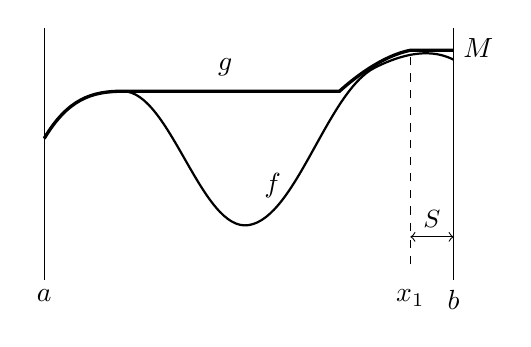
\begin{tikzpicture}[scale=1]
  \draw (0,-0.2) -- (0,3);
  \draw (5.2,-0.2) -- (5.2,3);
  \draw[thick] (0,1.6) .. controls (0.3,2.1) and (0.6,2.2) .. (1,2.2)
    .. controls (1.6,2.2) and (2,0.4) .. (2.6,0.5)
    .. controls (3.2,0.6) and (3.6,2.2) .. (4.2,2.5)
    .. controls (4.7,2.75) and (5,2.7) .. (5.2,2.6);
  \draw[very thick] (0,1.6) .. controls (0.3,2.1) and (0.6,2.2) .. (1,2.2) -- (3.75,2.2)
    .. controls (3.95,2.38) and (4.3,2.65) .. (4.65,2.72) -- (5.2,2.72);
  \node at (2.3,2.5) {$g$};
  \node at (2.9,1.0) {$f$};
  \node[right] at (5.2,2.75) {$M$};
  \draw[dashed] (4.65,0) -- (4.65,2.72);
  \draw[<->] (4.65,0.35) -- (5.2,0.35) node[midway,above] {\small$S$};
  \node[below] at (0,-0.2) {$a$};
  \node[below] at (4.65,-0.2) {$x_1$};
  \node[below] at (5.2,-0.2) {$b$};
\end{tikzpicture}
\end{center}

\begin{itemize}
  \item $g$ es monótona creciente,
  \item $g(a)=f(a)$,
  \item $g(b)=M$.
\end{itemize}
Sea $S:=\{x\in[a,b] : g(x)=M\}$. Tenemos que $b\in S$. Sea $x_1:=\inf(S)$.
\begin{itemize}
  \item Para todo $x<x_1$, $x\notin S$, entonces $g(x)<M$.
  \item Para todo $x>x_1$, existe $x'\in S$ tal que $x>x'>x_1\ (=\inf)$:
  \[
    g(x)\geq g(x')=M,
  \]
  entonces $g(x)=M$, $x\in S$.
  \item $S$ es un intervalo de la forma $S=(x_1,b]$ o $S=[x_1,b]$.
\end{itemize}

\begin{center}
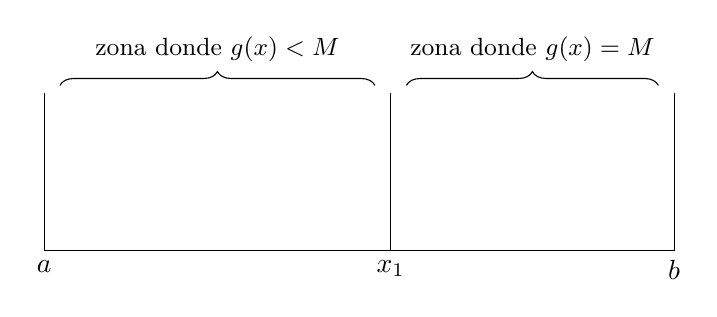
\begin{tikzpicture}
  \draw (0,0) -- (8,0);
  \draw (0,0) -- (0,2); \draw (4.4,0) -- (4.4,2); \draw (8,0) -- (8,2);
  \node[below] at (0,0) {$a$};
  \node[below] at (4.4,0) {$x_1$};
  \node[below] at (8,0) {$b$};
  \draw[decorate,decoration={brace,amplitude=5pt}] (0.2,2.1) -- (4.2,2.1) node[midway,above=5pt] {\small zona donde $g(x)<M$};
  \draw[decorate,decoration={brace,amplitude=5pt}] (4.6,2.1) -- (7.8,2.1) node[midway,above=5pt] {\small zona donde $g(x)=M$};
\end{tikzpicture}
\end{center}

Queremos mostrar que $f(x_1)=M$. Por el absurdo, se supone que $f(x_1)<M$.

Sea $\varepsilon:=\dfrac{M-f(x_1)}{2}>0$. Como $f$ es continua en $x_1$, existe $\delta>0$ tal que $\abs{f(x)-f(x_1)}<\varepsilon$ para todo $x\in E(x_1,\delta)\cap[a,b]$.

Para todo $x\in E(x_1,\delta)\cap[a,b]$,
\[
  f(x)<f(x_1)+\varepsilon = f(x_1)+\frac{M-f(x_1)}{2} = \frac{M+f(x_1)}{2} = M-\varepsilon.
\]
Se definen
\begin{align*}
  x_1^- &= \max\left(x_1-\frac\delta2,\ a\right),\\
  x_1^+ &= \min\left(x_1+\frac\delta2,\ b\right).
\end{align*}
\begin{align*}
  g(x_1^+) &= \sup\big(f,[a,x_1^+]\big)\\
  &= \sup\big(f,[a,x_1^-]\cup[x_1^-,x_1^+]\big)\\
  &= \max\Big(\sup\big(f,[a,x_1^-]\big),\ \sup\big(f,[x_1^-,x_1^+]\big)\Big)\\
  &= \max\Big(g(x_1^-),\ \sup\big(f,[x_1^-,x_1^+]\big)\Big) \leq \max\big(g(x_1^-),\ M-\varepsilon\big).
\end{align*}
Se distinguen 3 casos:

\textbf{Caso 1:} $a=x_1<b$. Tenemos que $a=x_1^-=x_1<x_1^+\leq b$.
\[
  \left.\begin{array}{l}
    g(x_1^+)=\sup\big(f,[a,x_1^+]\big)=\sup\big(f,[x_1^-,x_1^+]\big)\leq M-\varepsilon\\[2pt]
    \text{Por otro lado: } x_1^+>x_1, \text{ luego } g(x_1^+)=M
  \end{array}\right\}\ \text{Contradicción.}
\]

\textbf{Caso 2:} $a<x_1=b$. Tenemos que: $a\leq x_1^-<x_1=x_1^+=b$.
\[
  \left.\begin{array}{l}
    g(x_1^+)\leq\max\big(\underbrace{g(x_1^-)}_{<\,M},\ M-\varepsilon\big)<M\\[2pt]
    \text{Por otro lado: } g(x_1^+)=g(b)=M
  \end{array}\right\}\ \text{Contradicción.}
\]

\textbf{Caso 3:} $a<x_1<b$. Tenemos que $a\leq x_1^-<x_1<x_1^+\leq b$.
\[
  \left.\begin{array}{l}
    g(x_1^+)\leq\dots<M\\[2pt]
    \text{Por otro lado: } x_1^+>x_1, \text{ entonces } g(x_1^+)=M
  \end{array}\right\}\ \text{Contradicción.} \qedhere
\]
\end{demo}

\subsection{Funciones inversas}

\begin{proposicion}
Sea $f:A\to\R$ una función definida en un subconjunto $A\subset\R$. Si $f$ es estrictamente creciente o decreciente, entonces $f$ es inyectiva, y define una biyección entre $A$ y su imagen $B:=f(A)$ por la función $f$. Además, la función inversa $f^{-1}:B\to A$ también es estrictamente creciente (o decreciente).
\end{proposicion}

\begin{teorema}
Si $f:I\to\R$ es continua y estrictamente creciente (o decreciente), entonces es inyectiva, y define una biyección de $I$ a su imagen $J:=f(I)$ \comentario{$\leftarrow$ intervalo por Bolzano}. Además, la función inversa $f^{-1}:J\to I$ es continua y estrictamente creciente (o decreciente).
\end{teorema}

\begin{center}
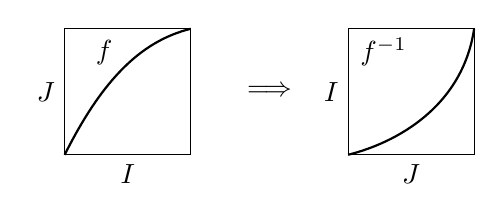
\begin{tikzpicture}
  \draw (0,0) rectangle (1.6,1.6);
  \draw[thick] (0,0) .. controls (0.5,1.0) and (1.0,1.45) .. (1.6,1.6);
  \node at (0.5,1.3) {$f$};
  \node[below] at (0.8,0) {$I$};
  \node[left] at (0,0.8) {$J$};
  \node at (2.6,0.8) {$\Longrightarrow$};
  \begin{scope}[xshift=3.6cm]
    \draw (0,0) rectangle (1.6,1.6);
    \draw[thick] (0,0) .. controls (0.6,0.15) and (1.45,0.6) .. (1.6,1.6);
    \node at (0.45,1.3) {$f^{-1}$};
    \node[below] at (0.8,0) {$J$};
    \node[left] at (0,0.8) {$I$};
  \end{scope}
\end{tikzpicture}
\end{center}

\begin{ejemplo}[Raíz $n$-ésima]
Sea $n\geq1$. Sea $f:[0,+\infty)\to[0,+\infty)$ definida por $f(x)=x^n$. $f$ es continua y estrictamente creciente. Se escribe
\[
  \sqrt[n]{x}:=f^{-1}(x),\qquad \sqrt[n]{\,\cdot\,}:[0,+\infty)\to[0,+\infty).
\]
Cuando $n$ es impar, se puede reemplazar $[0,+\infty)$ por $\R$.
\end{ejemplo}

\begin{ejemplo}
Sea $f:\R^+\to\R$, \ $x\mapsto f(x)=\log(x)$.
\begin{itemize}
  \item $f$ es estrictamente creciente y continua.
  \item $\displaystyle\lim_{x\to0^+}\log(x)=-\infty$ \ y \ $\displaystyle\lim_{x\to+\infty}\log(x)=+\infty$.
\end{itemize}
Luego: $\log(\R^+)=\R$.
\end{ejemplo}

\begin{definicion}
$\exp:=\log^{-1}:\R\to\R^+$.
\end{definicion}

\textbf{Propiedad:}
\[
  \exp(0)=1,\qquad \exp(x+y)=\exp(x)\exp(y),\qquad \exp(-x)=\frac{1}{\exp(x)}.
\]

Se define $e:=\exp(1)$.


% =====================================================================
% La hoja de la clase 26 no tiene fecha: el campo queda vacío.
\clase{26}{}{Exponencial y continuidad uniforme}

\subsection{Funciones inversas}

$f:I\to\R$ estrictamente creciente o decreciente y continua, entonces define una biyección entre $I$ y su imagen $J:=f(I)$. Además, la función inversa $f^{-1}:J\to I$ es continua y estrictamente creciente o decreciente.

\begin{ejemplo}
Sea $\log:\R_+\to\R$. Tenemos que
\[
  \lim_{x\to0^+}\log x=-\infty,\qquad \lim_{x\to+\infty}\log x=+\infty.
\]
$\log(\R_+)=\R$.

Se escribe $\exp:=\log^{-1}:\R\to\R^+$.
\end{ejemplo}

\begin{proposicion}
$\exp(x+y)=\exp(x)\exp(y)$.
\end{proposicion}

\begin{align*}
  \log\big(\exp(x+y)\big) &= x+y = \log\big(\exp(x)\big)+\log\big(\exp(y)\big)\\
  &= \log\big(\exp(x)\exp(y)\big)
\end{align*}
\[
  \implies \exp(x+y)=\exp(x)\exp(y).
\]
\[
  \exp(-x)=\frac{1}{\exp(x)}\qquad\qquad \exp(0)=1
\]

\begin{definicion}
Sea $e:=\exp(1)\simeq 2{,}718\ldots$ \quad ($\notin\Q$).
\end{definicion}

\begin{proposicion}
\[
  \exp n=\exp(\underbrace{1+\cdots+1}_{n})=\underbrace{e\times\cdots\times e}_{n}=e^n.
\]
\end{proposicion}

Por analogía, se escribe $e^x:=\exp(x)$.

\begin{proposicion}
\[
  e^{x+y}=e^xe^y\qquad\qquad e^0=1\qquad\qquad e^{-x}=\frac{1}{e^x}
\]
\end{proposicion}

\textbf{Potencia:}
\begin{align*}
  x\in\R,\ n\in\N &\leadsto x^n\\
  x\neq0,\ n\in\Z^- &\leadsto x^n=\frac{1}{x^{-n}}
\end{align*}
\begin{center}
\fbox{$x>0,\ y\in\R \leadsto x^y:=e^{y\log x}$}\\[0.2em]
Potencia generalizada
\end{center}

\subsection{Funciones definidas a partir de integrales}

\begin{proposicion}
Si $f:I\to\R$ es localmente integrable y $a\in I$, entonces la función $F:I\to\R$ definida por
\[
  F(x)=\int_a^x f(t)\dd t
\]
es continua.
\end{proposicion}

\begin{demo}
Sea $x_0\in I$. Como $f$ es localmente integrable, está acotada en un entorno de $x_0$, y existen $\delta>0$ y $M\geq0$ tales que
\[
  \forall x\in E(x_0,\delta),\quad \abs{f(x)}\leq M.
\]
Para todo $x\in E(x_0,\delta)$:
\begin{align*}
  \abs{F(x)-F(x_0)} &= \abs*{\int_a^x f-\int_a^{x_0} f} = \abs*{\int_{x_0}^x f}\\
  &\leq \int_{\min(x,x_0)}^{\max(x,x_0)}\abs{f} \leq M\cdot\abs{x-x_0}\xrightarrow[x\to x_0]{}0.
\end{align*}
Por el sándwich:
\[
  \abs{F(x)-F(x_0)}\xrightarrow[x\to x_0]{}0,\qquad F(x)\xrightarrow[x\to x_0]{}F(x_0). \qedhere
\]
\end{demo}

\begin{center}
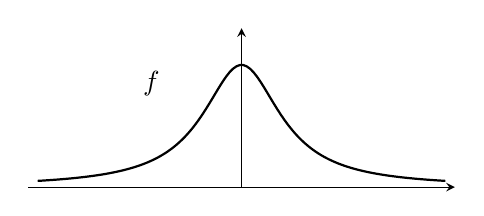
\begin{tikzpicture}
  \begin{axis}[
    width=7cm, height=3.6cm,
    axis lines=middle, xmin=-4.5, xmax=4.5, ymin=0, ymax=1.3,
    xtick={0}, ytick=\empty, samples=120, domain=-4.3:4.3,
    clip=false]
    \addplot[thick] {1/(1+x^2)};
    \node at (axis cs:-1.9,0.85) {$f$};
  \end{axis}
\end{tikzpicture}
\qquad
$\displaystyle f(t)=\frac{1}{1+t^2}$
\qquad
$\displaystyle F(x)=\int_0^x\frac{1}{1+t^2}\dd t$
\end{center}

\subsection{Continuidad uniforme}

\begin{ejemplo}
Sea $f:\R^+\to\R$ def.\ por $f(x)=x^2$. Sean $x_0>0$ y $\varepsilon>0$ tal que $\varepsilon\leq x_0^2$.

Determinar el máximo $\delta>0$ tal que
\[
  \forall x\in\R^+,\quad \abs{x-x_0}<\delta\implies\abs{x^2-x_0^2}<\varepsilon.
\]

\begin{center}
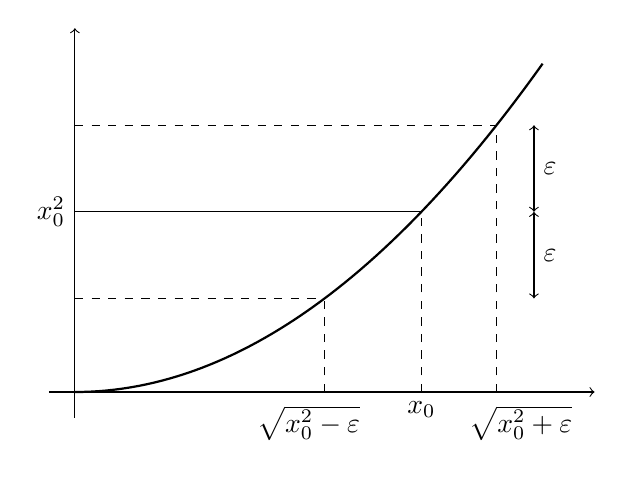
\begin{tikzpicture}[scale=1.1]
  \draw[->] (-0.3,0) -- (6,0);
  \draw[->] (0,-0.3) -- (0,4.2);
  \draw[thick,domain=0:5.4,samples=60] plot (\x,{0.13*\x*\x});
  % x0 = 4  -> x0^2 = 2.08 ; eps = 1.0
  \draw (0,2.08) -- (4,2.08);
  \draw[dashed] (4,0) -- (4,2.08);
  \draw[dashed] (0,1.08) -- (2.88,1.08);
  \draw[dashed] (0,3.08) -- (4.87,3.08);
  \draw[dashed] (2.88,0) -- (2.88,1.08);
  \draw[dashed] (4.87,0) -- (4.87,3.08);
  \node[below] at (4,0) {$x_0$};
  \node[below] at (2.7,-0.05) {$\sqrt{x_0^2-\varepsilon}$};
  \node[below] at (5.15,-0.05) {$\sqrt{x_0^2+\varepsilon}$};
  \node[left] at (0,2.08) {$x_0^2$};
  \draw[<->] (5.3,2.08) -- (5.3,3.08) node[midway,right] {$\varepsilon$};
  \draw[<->] (5.3,1.08) -- (5.3,2.08) node[midway,right] {$\varepsilon$};
\end{tikzpicture}
\end{center}

\begin{align*}
  \abs{x^2-x_0^2}<\varepsilon &\iff x_0^2-\varepsilon<x^2<x_0^2+\varepsilon\\
  &\iff \sqrt{x_0^2-\varepsilon}<x<\sqrt{x_0^2+\varepsilon}
\end{align*}
$\delta>0$ debe cumplir
\begin{align*}
  \delta &\leq x_0-\sqrt{x_0^2-\varepsilon}\\
  \delta &\leq \sqrt{x_0^2+\varepsilon}-x_0 \quad\text{\comentario{$\longleftarrow$ más restrictiva}}
\end{align*}
El radio máximo es $\delta:=\sqrt{x_0^2+\varepsilon}-x_0$.
\end{ejemplo}

\textbf{Moraleja:} $\delta$ depende de $\varepsilon$ y de $x_0$.

\begin{definicion}
Una función $f:I\to\R$ es uniformemente continua en $I$ cuando:
\[
  \forall\varepsilon>0,\ \exists\delta>0,\ \forall x,x'\in I,\quad \abs{x-x'}<\delta\implies\abs{f(x)-f(x')}<\varepsilon.
\]
\end{definicion}

\begin{proposicion}
Toda función uniformemente continua es continua.
\end{proposicion}

\begin{demo}
\begin{align*}
  &f \text{ uniformemente continua}\\
  \iff{}& \forall\varepsilon>0,\ \exists\delta>0,\ \forall x,x'\in I,\ \abs{x-x'}<\delta\implies\abs{f(x)-f(x')}<\varepsilon\\
  \implies{}& \forall\varepsilon>0,\ \forall x\in I,\ \exists\delta>0,\ \forall x'\in I,\ \abs{x-x'}<\delta\implies\abs{f(x)-f(x')}<\varepsilon\\
  \iff{}& \forall x\in I,\ \forall\varepsilon>0,\ \exists\delta>0,\ \forall x'\in I,\ \abs{x-x'}<\delta\implies\abs{f(x)-f(x')}<\varepsilon \qedhere
\end{align*}
\end{demo}

\begin{contraejemplo}
$f(x)=x^2$ en $\R$.

Supongamos que $f(x)=x^2$ es uniformemente continua en $\R$. Fijando $\varepsilon>0$,
\[
  \exists\delta>0,\ \forall x,x'\in\R,\quad \abs{x-x'}<\delta\implies\abs{x^2-x'^2}<\varepsilon.
\]
Fijando $x>0$, tenemos que
\[
  \forall x'\in\R,\quad \abs{x'-x}<\delta\implies\abs{x^2-x'^2}<\varepsilon.
\]
Entonces tenemos que $\delta\leq\sqrt{x^2+\varepsilon}-x$ \ $\forall x$.
\begin{align*}
  \delta\leq\sqrt{x^2+\varepsilon}-x
  &= \frac{\big(\sqrt{x^2+\varepsilon}-x\big)\big(\sqrt{x^2+\varepsilon}+x\big)}{\sqrt{x^2+\varepsilon}+x}\\
  &= \frac{x^2+\varepsilon-x^2}{\sqrt{x^2+\varepsilon}+x}
   = \frac{\varepsilon}{\sqrt{x^2+\varepsilon}+x}\xrightarrow[x\to+\infty]{}0.
\end{align*}
Luego: $\delta\leq0$. Contradicción, pues $\delta>0$.
\end{contraejemplo}

\[
  \text{Continuidad uniforme}\ \mathrel{\begin{array}{@{}c@{}}\Longrightarrow\\[-0.3em] \cancel{\Longleftarrow}\end{array}}\ \text{continuidad}
\]

Cuando el intervalo es de la forma $[a,b]$ entonces ambas definiciones son equivalentes.

\begin{teorema}[Heine--Cantor]
Toda función continua en un intervalo cerrado $[a,b]$ es uniformemente continua en $[a,b]$.
\end{teorema}


% =====================================================================
% La hoja de la clase 27 no tiene fecha: el campo queda vacío.
\clase{27}{}{Heine--Cantor e integrabilidad}

\subsection{Continuidad uniforme}

$f:I\to\R$ es uniformemente continua en $I$
\[
  \iff \forall\varepsilon>0,\ \exists\delta>0,\ \forall x,x'\in I,\quad \abs{x-x'}<\delta\implies\abs{f(x)-f(x')}<\varepsilon
\]
$f:I\to\R$ es continua
\[
  \iff \forall x\in I,\ \forall\varepsilon>0,\ \exists\delta>0,\ \forall x'\in I,\quad \abs{x'-x}<\delta\implies\abs{f(x')-f(x)}<\varepsilon
\]

\subsection{Teorema de Heine--Cantor}

\textbf{Objetivo:} Demostrar que toda función continua $[a,b]$ (cerrado) es uniformemente continua.

\begin{lema}
Sea $h:[a,b]\to\R^+$ (función positiva cualquiera). Entonces, existe una sucesión finita de puntos $x_1,\dots,x_n\in[a,b]$ tales que los entornos $E(x_1,h(x_1)),\dots,E(x_n,h(x_n))$ cubren el intervalo $[a,b]$:
\[
  [a,b]\subset E(x_1,h(x_1))\cup\cdots\cup E(x_n,h(x_n)).
\]
\end{lema}

\begin{observacion}
Si $r>0$ se puede cubrir $[a,b]$ con finitos entornos de radio $r$: basta con tomar $n$ tal que $2rn>b-a$.
\end{observacion}

\begin{demo}
Dado un subintervalo $[c,d]\subset[a,b]$, se llama un $h$-cubrimiento de $[c,d]$ a toda sucesión $x_1,\dots,x_n\in[c,d]$ tal que
\[
  [c,d]\subset E(x_1,h(x_1))\cup\cdots\cup E(x_n,h(x_n)).
\]
Sea $A:=\{c\in[a,b] : \exists \text{ un } h\text{-cubrimiento de } [a,c]\}$.

Por construcción: $a\in A$ pues $[a,a]=\{a\}\subset E(a,h(a))$.

Sea $s:=\sup(A)$ \ $(\in[a,b])$.
\begin{enumerate}[label=(\arabic*)]
  \item $a\in A$
  \item $s:=\sup(A)$
  \item Como $s=\sup(A)$, existe $c\in A$ tal que $s-h(s)<c\leq s$.

  Como $c\in A$, existen $x_1,\dots,x_n\in[a,c]$ tales que
  \[
    [a,c]\subset E(x_1,h(x_1))\cup\cdots\cup E(x_n,h(x_n)).
  \]
  \item Por construcción: $\abs{s-c}<h(s)$: \ $c\in E(s,h(s))$, \ $[c,s]\subset E(s,h(s))$.

  El punto $s$ es un $h$-cubrimiento de $[c,s]$.
  \item Pegando los dos $h$-cubrimientos: la sucesión $x_1,\dots,x_n,s$ \comentario{con $n+1$ elementos} es un $h$-cubrimiento de $[a,s]$: luego $s\in A$.
  \item Por el absurdo, supongamos que $s<b$. Sea
  \[
    s':=\min\left(s+\frac{h(s)}{2},\ b\right)>s.
  \]
  Por construcción $[s,s']\subset E(s,h(s))$.

  Luego, la sucesión $x_1,\dots,x_n,s$ es un $h$-cubrimiento de
  \[
    [a,s]\cup[s,s']=[a,s'].
  \]
  Luego: $s'\in A$. Absurdo, pues $s'>s=\sup(A)$.
\end{enumerate}
Por lo tanto $s=b\in A$.
\end{demo}

\begin{teorema}[Heine--Cantor]
Toda función continua en un intervalo cerrado $[a,b]$ es uniformemente continua en $[a,b]$.
\end{teorema}

\begin{demo}
$f:[a,b]\to\R$. Sea $\varepsilon>0$, se trata de hallar un $\delta'>0$ uniforme tal que
\[
  \forall x,x'\in[a,b],\quad \abs{x-x'}<\delta'\implies\abs{f(x)-f(x')}<\varepsilon.
\]
Como $f$ es continua, para todo punto $x\in[a,b]$, existe $\delta_x>0$ tal que
\[
  \forall x'\in[a,b],\quad \abs{x-x'}<\delta_x\implies\abs{f(x)-f(x')}<\varepsilon/2.
\]
Sea $h:[a,b]\to\R^+$ definida por $h(x)=\delta_x/2$.

Por el lema, existen $x_1,\dots,x_n\in[a,b]$ tales que
\[
  E(x_1,h(x_1))\cup\cdots\cup E(x_n,h(x_n))\supset[a,b].
\]
Sea
\[
  \delta':=\min\big(h(x_1),\dots,h(x_n)\big)=\frac12\min\big(\delta_{x_1},\dots,\delta_{x_n}\big)>0.
\]
Se trata de demostrar:
\[
  \forall x,x'\in[a,b],\quad \abs{x-x'}<\delta'\implies\abs{f(x)-f(x')}<\varepsilon.
\]
Sean $x,x'\in[a,b]$ tales que $\abs{x-x'}<\delta'$. Como $E(x_1,h(x_1))\cup\cdots\cup E(x_n,h(x_n))$ $\supset$ $[a,b]$, existe $i$ (entre $1$ y $n$) tal que $x\in E(x_i,h(x_i))=E(x_i,\delta_{x_i}/2)$.
\[
  \abs{x-x_i}<\delta_{x_i}/2<\delta_{x_i},\quad\text{luego}\quad \abs{f(x)-f(x_i)}<\varepsilon/2.
\]
Además:
\[
  \abs{x'-x_i}\leq\abs{x'-x}+\abs{x-x_i}<\delta'+h(x_i)\leq2h(x_i)=\delta_{x_i},
\]
luego $\abs{f(x')-f(x_i)}<\varepsilon/2$.

Por lo tanto:
\[
  \abs{f(x)-f(x')}\leq\abs{f(x)-f(x_i)}+\abs{f(x')-f(x_i)}<\frac\varepsilon2+\frac\varepsilon2=\varepsilon. \qedhere
\]
\end{demo}

\subsubsection*{Consecuencia}

\begin{proposicion}
Toda función continua $f$ en $[a,b]$ es integrable en $[a,b]$.
\end{proposicion}

\begin{demo}
Se usa el criterio de integrabilidad a menos de $\varepsilon$.

Fijando $\varepsilon>0$, queremos construir una partición $P\subset[a,b]$ tal que
\[
  S^*(f,P)-S_*(f,P)<\varepsilon.
\]
Se elige $\eta>0$ tal que $\eta<\dfrac{\varepsilon}{b-a}$ $(>0)$. Por ejemplo $\eta:=\dfrac{\varepsilon}{2(b-a)}$.

Como $f$ es continua en $[a,b]$, es uniformemente continua. Sea $\delta>0$ tal que
\[
  \forall x,x'\in[a,b],\quad \abs{x-x'}<\delta\implies\abs{f(x)-f(x')}<\eta.
\]
Sea $P\subset[a,b]$ tal que $\norm{P}<\delta$.

En cada subintervalo $[a_i,a_{i+1}]$ se observa: como $\forall x,x'\in[a_i,a_{i+1}]$, $f(x)-f(x')<\eta$. Esto implica que
\[
  \sup\big(f,[a_i,a_{i+1}]\big)-\inf\big(f,[a_i,a_{i+1}]\big)\leq\eta.
\]
Tenemos que
\begin{align*}
  S^*(f,P)-S_*(f,P) &= \sum_{i=0}^{n-1}(a_{i+1}-a_i)\times\Big(\sup\big(f,[a_i,a_{i+1}]\big)-\inf\big(f,[a_i,a_{i+1}]\big)\Big)\\
  &\leq \sum_{i=0}^{n-1}(a_{i+1}-a_i)\cdot\eta = \eta\cdot\sum_{i=0}^{n-1}(a_{i+1}-a_i)\\
  &= \eta(b-a)\\
  &< \frac{\varepsilon}{b-a}\times(b-a)=\varepsilon. \qedhere
\end{align*}
\end{demo}


% =====================================================================
% La hoja de la clase 28 no tiene fecha: el campo queda vacío.
% Última clase de la unidad. La segunda mitad de la clase 28 (funciones
% trigonométricas) está en CDIV-Trigonometria.tex.
\clase{28}{}{Continuidad seccional y valor medio}

\subsection{Continuidad uniforme}

\begin{corolario}
Toda función continua en un intervalo $I$ (cualquiera) es localmente integrable en $I$.
\end{corolario}

\begin{definicion}
Una función $f:[a,b]\to\R$ es \emph{seccionalmente continua} cuando existe una partición $P\subset[a,b]$ tal que para todo $i=0,\dots,n-1$ \comentario{$P=\{a_0,a_1,\dots,a_n\}$}:
\begin{enumerate}[label=(\arabic*)]
  \item $f$ es continua en $(a_i,a_{i+1})$ (abierto).
  \item En $(a_i,a_{i+1})$, $f$ tiene límites finitos en $a_i$ (por la derecha) y en $a_{i+1}$ (por la izquierda).
\end{enumerate}
\end{definicion}

\begin{proposicion}
Toda función seccionalmente continua en $[a,b]$ es integrable en $[a,b]$.
\end{proposicion}

\begin{definicion}[Valor medio]
Sea $f:[a,b]\to\R$ una función integrable. Se define su valor medio por
\[
  \mu:=\frac{1}{b-a}\int_a^b f(x)\dd x.
\]
\end{definicion}

\subsection{Teorema del valor medio}

\begin{teorema}[Teorema del valor medio]
Si $f:[a,b]\to\R$ es continua, entonces alcanza su valor medio:
\[
  \exists c\in[a,b],\qquad f(c)=\mu=\frac{1}{b-a}\int_a^b f(x)\dd x.
\]
\end{teorema}

\begin{demo}
Como $f$ continua en $[a,b]$, existen $x_0,x_1\in[a,b]$ tales que $\forall x\in[a,b]$
\[
  \underbrace{f(x_0)}_{m}\leq f(x)\leq\underbrace{f(x_1)}_{M}.
\]
$\forall x\in[a,b]$:
\begin{gather*}
  m\leq f(x)\leq M\\
  m(b-a)\leq\int_a^b f(x)\dd x\leq M(b-a)\\
  \underbrace{m}_{f(x_0)}\leq\underbrace{\frac{1}{b-a}\int_a^b f(x)\dd x}_{\mu}\leq\underbrace{M}_{f(x_1)}
\end{gather*}
Por el teorema de los valores intermedios, existe $c\in[x_0,x_1]$ (o $[x_1,x_0]$) tal que $f(c)=\mu$.
\end{demo}

\begin{contraejemplo}
$f(x)=\lfloor x\rfloor$ en $[0,2]$.

\begin{center}
\begin{tikzpicture}[scale=1.3]
  \draw[->] (-0.2,0) -- (2.6,0);
  \draw[->] (0,-0.2) -- (0,2.4);
  \foreach \y in {1,2} \draw (-0.05,\y) -- (0.05,\y) node[left=3pt] {\small$\y$};
  \foreach \x in {1,2} \draw (\x,-0.05) -- (\x,0.05) node[below=5pt] {\small$\x$};
  \node[below left] at (0,0) {\small$0$};
  % escalones
  \draw[very thick] (0,0) -- (1,0);
  \fill (0,0) circle (1.6pt);
  \draw[fill=white] (1,0) circle (1.6pt);
  \draw[very thick] (1,1) -- (2,1);
  \fill (1,1) circle (1.6pt);
  \draw[fill=white] (2,1) circle (1.6pt);
  \fill (2,2) circle (1.6pt);
  % valor medio
  \draw[dashed] (0,0.5) -- (2,0.5) node[right] {$\mu=\frac12$};
\end{tikzpicture}
\qquad\qquad
$\displaystyle\frac12\int_0^2\lfloor x\rfloor\dd x=\frac12$
\end{center}
\end{contraejemplo}


% =====================================================================
\end{document}
